\section{Full Experimental Results}
\label{app:full_results}

This appendix provides complete numerical results for all 22 models evaluated in our experiments. \Cref{tab:cifar_full} reports the full CIFAR-10 results and \Cref{tab:imagenet_full} reports the ImageNet results. \Cref{tab:per_class_cifar} provides the per-class GREAT Score breakdown for all CIFAR-10 models.

\begin{table}[H]
    \caption{Full GF-Score results for 17 CIFAR-10 $\ell_2$ models, sorted by RobustBench accuracy. \textbf{RB Acc}: RobustBench robust accuracy (\%). \textbf{GS}: uncalibrated GREAT Score. \textbf{Cal.\ GS}: calibrated GREAT Score ($T^* = 2.70$). \textbf{FP-GR}: Fairness-Penalized GREAT ($\lambda = 0.5$).}
    \label{tab:cifar_full}
    \centering
    \scriptsize
    \begin{tabular}{@{}lrrrrrrlr@{}}
        \toprule
        \textbf{Model} & \textbf{RB Acc} & \textbf{GS} & \textbf{Cal.\ GS} & \textbf{RDI} & \textbf{NRGC} & \textbf{WCR} & \textbf{WCR Class} & \textbf{FP-GR} \\
        \midrule
        Rebuffi\_extra     & 82.32 & 0.465 & 0.330 & 0.333 & 0.135 & 0.283 & cat & 0.298 \\
        Gowal\_extra       & 80.53 & 0.480 & 0.344 & 0.348 & 0.138 & 0.288 & cat & 0.306 \\
        Rebuffi\_70\_ddpm  & 80.42 & 0.381 & 0.277 & 0.360 & 0.178 & 0.166 & cat & 0.201 \\
        Augustin\_WRN\_ext & 78.79 & 0.526 & 0.330 & 0.319 & 0.105 & 0.335 & cat & 0.366 \\
        Rebuffi\_28\_ddpm  & 78.80 & 0.352 & 0.255 & 0.359 & 0.191 & 0.144 & cat & 0.173 \\
        Sehwag\_Proxy      & 77.24 & 0.232 & 0.290 & 0.302 & 0.250 & 0.060 & cat & 0.081 \\
        Augustin\_WRN      & 76.25 & 0.483 & 0.309 & 0.385 & 0.135 & 0.242 & cat & 0.291 \\
        Rade\_R18          & 76.15 & 0.337 & 0.256 & 0.315 & 0.177 & 0.157 & cat & 0.179 \\
        Rebuffi\_R18       & 75.86 & 0.302 & 0.220 & 0.326 & 0.193 & 0.121 & cat & 0.139 \\
        Gowal2020          & 74.50 & 0.111 & 0.207 & 0.121 & 0.192 & 0.046 & dog & 0.050 \\
        Sehwag\_R18        & 74.41 & 0.186 & 0.257 & 0.248 & 0.258 & 0.054 & cat & 0.062 \\
        Wu2020             & 73.66 & 0.105 & 0.173 & 0.111 & 0.194 & 0.047 & dog & 0.049 \\
        Augustin2020       & 72.91 & 0.488 & 0.304 & 0.435 & 0.142 & 0.218 & cat & 0.271 \\
        Engstrom2019       & 69.24 & 0.126 & 0.252 & 0.234 & 0.327 & 0.024 & dog & 0.009 \\
        Rice2020           & 67.68 & 0.117 & 0.212 & 0.200 & 0.309 & 0.031 & dog & 0.017 \\
        Rony2019           & 66.44 & 0.222 & 0.324 & 0.275 & 0.225 & 0.096 & cat & 0.085 \\
        Ding\_MMA          & 66.09 & 0.086 & 0.235 & 0.127 & 0.218 & 0.039 & cat & 0.023 \\
        \bottomrule
    \end{tabular}
\end{table}

\begin{table}[H]
    \caption{Full GF-Score results for 5 ImageNet $\ell_\infty$ models, sorted by RobustBench accuracy. Calibrated at $T^* = 0.10$. Two models achieve $\mathrm{WCR} = 0.000$, indicating at least one class with zero certified robustness.}
    \label{tab:imagenet_full}
    \centering
    \small
    \begin{tabular}{@{}lrrrrrrlr@{}}
        \toprule
        \textbf{Model} & \textbf{RB Acc} & \textbf{GS} & \textbf{Cal.\ GS} & \textbf{RDI} & \textbf{NRGC} & \textbf{WCR} & \textbf{WCR Class} & \textbf{FP-GR} \\
        \midrule
        Salman\_WRN50-2 & 38.14 & 0.545 & 0.800 & 1.231 & 0.299 & 0.009 & n01756291 & $-$0.070 \\
        Salman\_R50     & 34.96 & 0.444 & 0.730 & 1.198 & 0.350 & 0.003 & n04525038 & $-$0.155 \\
        Engstrom2019    & 29.22 & 0.446 & 0.717 & 1.196 & 0.361 & 0.003 & n03710637 & $-$0.152 \\
        Wong2020        & 26.24 & 0.360 & 0.591 & 1.148 & 0.388 & 0.000 & n04525038 & $-$0.214 \\
        Salman\_R18     & 25.32 & 0.280 & 0.575 & 1.126 & 0.454 & 0.000 & n04525038 & $-$0.283 \\
        \bottomrule
    \end{tabular}
\end{table}

\begin{table}[H]
    \caption{Per-class GREAT Scores for all 17 CIFAR-10 $\ell_2$ models (uncalibrated, $T = 1.0$). The class ``cat'' (column 4) is consistently the lowest-scoring class, while ``automobile'' (column 2) is consistently the highest. The final column shows the aggregate score, which equals the weighted mean of per-class scores with zero numerical error.}
    \label{tab:per_class_cifar}
    \centering
    \scriptsize
    \setlength{\tabcolsep}{3pt}
    \begin{tabular}{@{}lcccccccccc|c@{}}
        \toprule
        \textbf{Model} & \rotatebox{70}{airplane} & \rotatebox{70}{auto} & \rotatebox{70}{bird} & \rotatebox{70}{cat} & \rotatebox{70}{deer} & \rotatebox{70}{dog} & \rotatebox{70}{frog} & \rotatebox{70}{horse} & \rotatebox{70}{ship} & \rotatebox{70}{truck} & \rotatebox{70}{Agg.} \\
        \midrule
        Aug.\_WRN\_ext & .579 & .654 & .463 & .335 & .430 & .444 & .518 & .598 & .613 & .621 & .526 \\
        Aug.\_WRN      & .486 & .628 & .435 & .242 & .404 & .346 & .548 & .577 & .584 & .585 & .483 \\
        Aug.2020       & .526 & .652 & .440 & .218 & .419 & .336 & .537 & .582 & .584 & .588 & .488 \\
        Ding\_MMA      & .084 & .128 & .074 & .039 & .064 & .047 & .090 & .166 & .090 & .080 & .086 \\
        Engstrom       & .115 & .232 & .092 & .038 & .077 & .024 & .102 & .168 & .158 & .258 & .126 \\
        Gowal2020      & .112 & .122 & .082 & .061 & .098 & .046 & .118 & .167 & .153 & .146 & .111 \\
        Gowal\_ext     & .549 & .636 & .391 & .288 & .349 & .368 & .459 & .591 & .570 & .598 & .480 \\
        Rade\_R18      & .373 & .472 & .244 & .157 & .238 & .211 & .375 & .420 & .437 & .441 & .337 \\
        Reb.\_28\_ddpm & .391 & .502 & .265 & .144 & .248 & .201 & .396 & .445 & .461 & .468 & .352 \\
        Reb.\_70\_ddpm & .414 & .527 & .302 & .166 & .282 & .221 & .430 & .478 & .493 & .499 & .381 \\
        Reb.\_extra    & .528 & .616 & .373 & .283 & .341 & .368 & .441 & .562 & .553 & .582 & .465 \\
        Reb.\_R18      & .324 & .447 & .227 & .121 & .215 & .176 & .343 & .387 & .398 & .379 & .302 \\
        Rice2020       & .107 & .200 & .074 & .031 & .079 & .031 & .107 & .151 & .156 & .231 & .117 \\
        Rony2019       & .212 & .370 & .193 & .096 & .107 & .129 & .232 & .298 & .306 & .278 & .222 \\
        Sehwag\_Proxy  & .227 & .277 & .201 & .060 & .154 & .072 & .341 & .363 & .313 & .317 & .232 \\
        Sehwag\_R18    & .197 & .233 & .129 & .054 & .115 & .061 & .261 & .302 & .272 & .240 & .186 \\
        Wu2020         & .104 & .134 & .078 & .062 & .091 & .047 & .097 & .158 & .116 & .158 & .105 \\
        \bottomrule
    \end{tabular}
\end{table}

\section{Additional Figures}
\label{app:figures}

This section presents additional visualizations referenced in the main text. All figures are generated from the same evaluation data reported in \Cref{app:full_results}.

\subsection{Disparity Bar Charts}
\label{app:disparity_bars}

\Cref{fig:disparity_bars} shows per-model RDI, NRGC, WCR, and FP-GREAT values as bar charts, providing an intuitive comparison of disparity across models within each dataset.

\begin{figure}[H]
    \centering
    \subfloat[CIFAR-10 ($\ell_2$, 17 models)]{%
        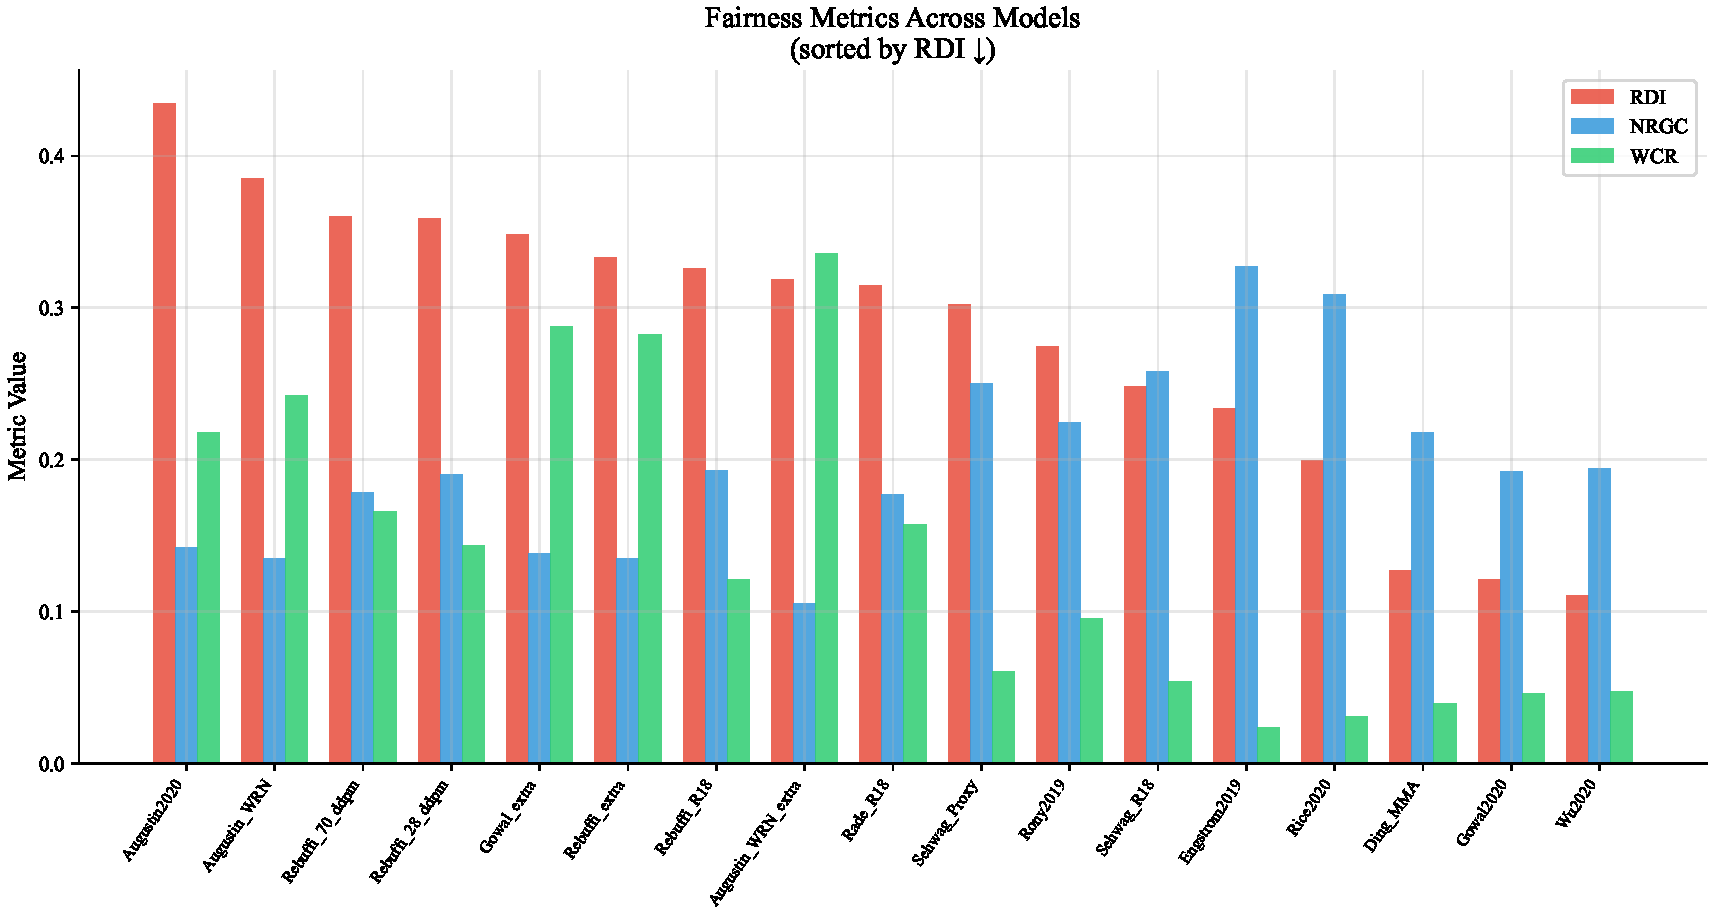
\includegraphics[width=0.48\linewidth]{figures/cifar/disparity_bars.pdf}%
    }\hfill
    \subfloat[ImageNet ($\ell_\infty$, 5 models)]{%
        
\includegraphics[width=0.48\linewidth]{figures/imagenet/disparity_bars.pdf}%
    }
    \caption{Disparity metric bar charts. Models are sorted by aggregate GREAT Score. Higher RDI and NRGC indicate greater disparity; lower WCR indicates worse fairness. All ImageNet models exhibit high RDI ($> 1.1$) due to the extreme class diversity (1{,}000 classes).}
    \label{fig:disparity_bars}
\end{figure}

\subsection{Vulnerability Analysis}
\label{app:vulnerability}

\Cref{fig:vulnerability} visualizes which classes are most and least robust across all models.

\begin{figure}[H]
    \centering
    \subfloat[CIFAR-10]{%
        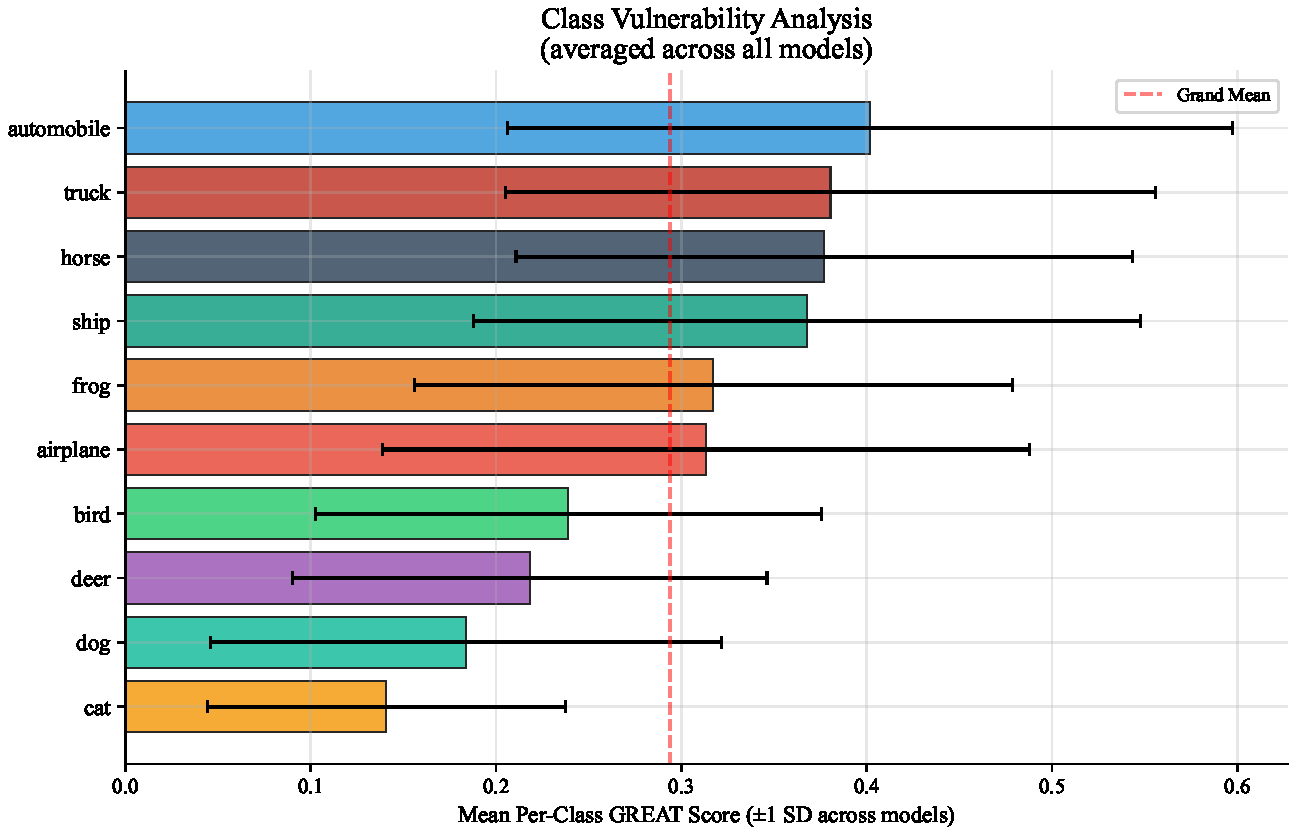
\includegraphics[width=0.48\linewidth]{figures/cifar/vulnerability.pdf}%
    }\hfill
    \subfloat[ImageNet]{%
        
\includegraphics[width=0.48\linewidth]{figures/imagenet/vulnerability.pdf}%
    }
    \caption{Class vulnerability analysis. On CIFAR-10, ``cat'' appears as the worst-case class in 13 of 17 models (76\%), while ``automobile'' is the best class in 10 of 17 (59\%). On ImageNet, ``n04525038'' (viaduct) is worst in 3 of 5 models, while ``n12057211'' (cattail) is best in all 5.}
    \label{fig:vulnerability}
\end{figure}

\subsection{FP-GREAT Rankings}
\label{app:fp_great_ranking}

\Cref{fig:fp_ranking} shows how model rankings change when using FP-GREAT ($\lambda = 0.5$) instead of the aggregate GREAT Score. Models with high disparity are penalized and drop in the fairness-aware ranking.

\begin{figure}[H]
    \centering
    \subfloat[CIFAR-10]{%
        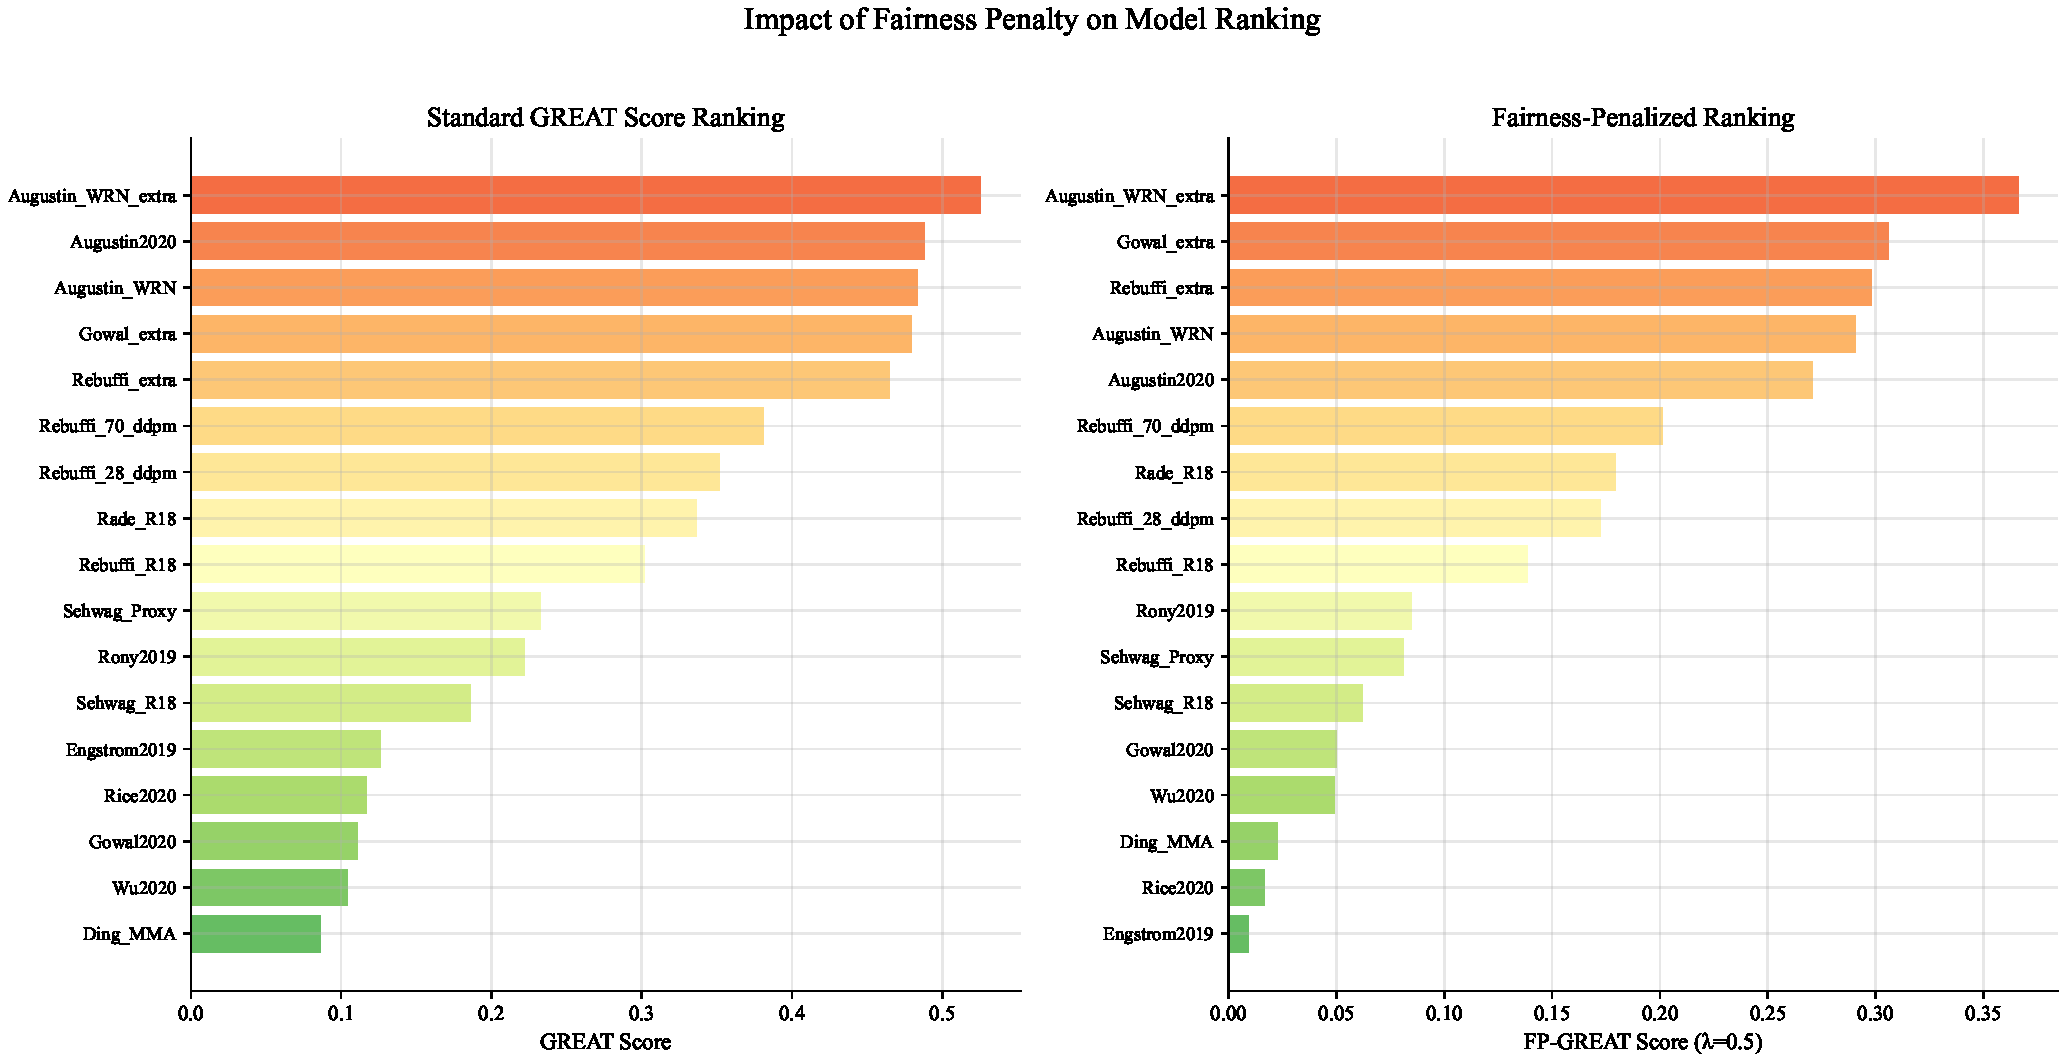
\includegraphics[width=0.48\linewidth]{figures/cifar/fp_great_ranking.pdf}%
    }\hfill
    \subfloat[ImageNet]{%
        
\includegraphics[width=0.48\linewidth]{figures/imagenet/fp_great_ranking.pdf}%
    }
    \caption{FP-GREAT re-ranking. On CIFAR-10, models with low disparity (e.g., Wu2020) rise, while those with high disparity (e.g., Augustin2020) fall. On ImageNet, the high RDI values ($> 1.1$) cause all FP-GREAT scores to be negative at $\lambda = 0.5$.}
    \label{fig:fp_ranking}
\end{figure}

\subsection{Self-Calibration Curves}
\label{app:calibration_curves}

\Cref{fig:calibration} plots the Spearman rank correlation as a function of temperature $T$ during the self-calibration grid search.

\begin{figure}[H]
    \centering
    \subfloat[CIFAR-10 ($T^* = 2.70$, $\rho = 0.871$)]{%
        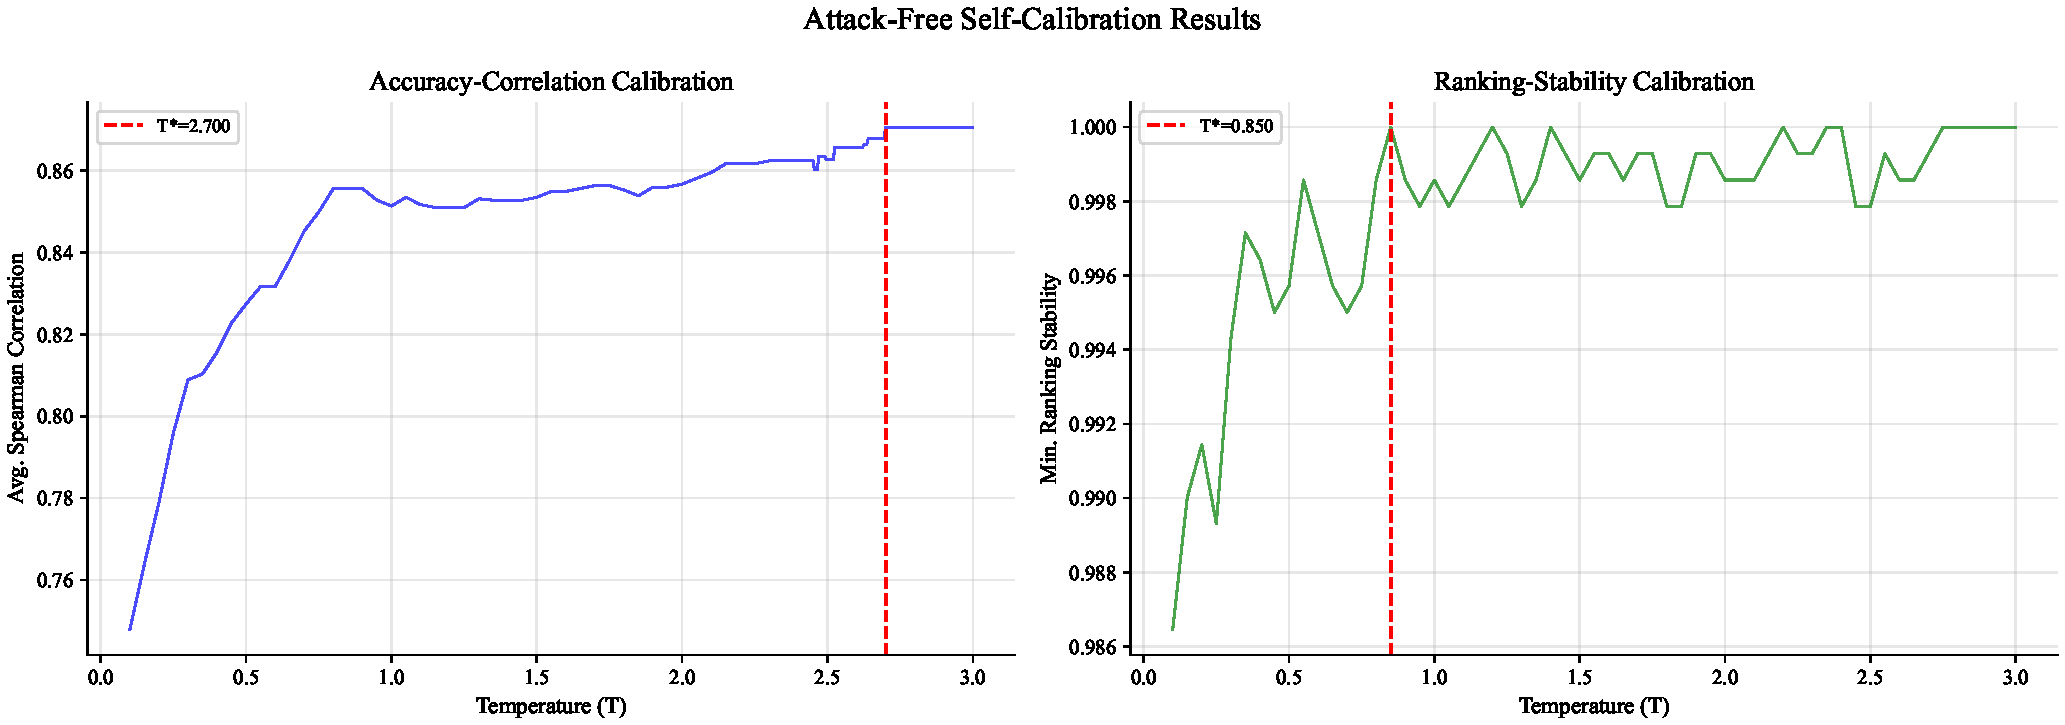
\includegraphics[width=0.48\linewidth]{figures/cifar/calibration.pdf}%
    }\hfill
    \subfloat[ImageNet ($T^* = 0.10$, $\rho = 1.000$)]{%
        
\includegraphics[width=0.48\linewidth]{figures/imagenet/calibration.pdf}%
    }
    \caption{Self-calibration curves. Both curves are smooth, confirming that the two-phase grid search reliably finds the optimum. On ImageNet, perfect agreement with RobustBench rankings is achieved using only clean accuracies.}
    \label{fig:calibration}
\end{figure}

\subsection{RDI Concentration Bounds}
\label{app:rdi_concentration}

\Cref{fig:rdi_concentration} visualizes the RDI concentration bound from \Cref{prop:rdi_concentration} as a function of per-class sample size $n_k$.

\begin{figure}[H]
    \centering
    \subfloat[CIFAR-10 ($K = 10$, $\delta = 0.05$)]{%
        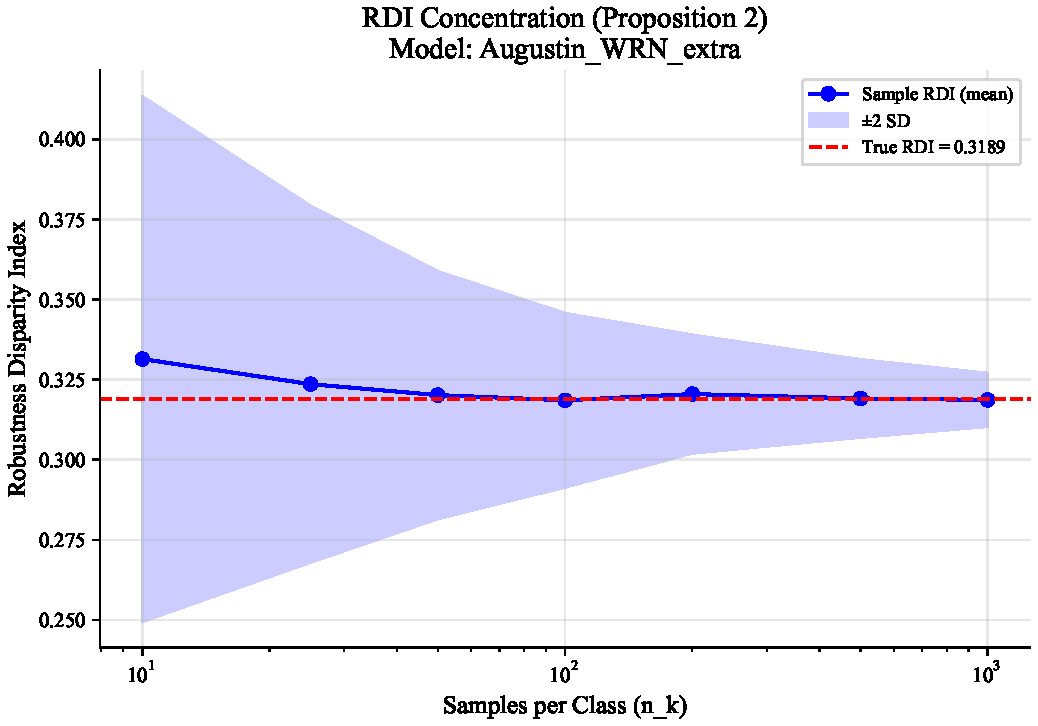
\includegraphics[width=0.48\linewidth]{figures/cifar/rdi_concentration.pdf}%
    }\hfill
    \subfloat[ImageNet ($K = 1{,}000$, $\delta = 0.05$)]{%
        
\includegraphics[width=0.48\linewidth]{figures/imagenet/rdi_concentration.pdf}%
    }
    \caption{RDI concentration bounds. The bound tightens as per-class sample size increases. Our CIFAR-10 evaluation with 1{,}000 samples per class provides tight estimates; the ImageNet union bound over 1{,}000 classes requires more samples, but 50 per class still achieves a bound of approximately 0.35.}
    \label{fig:rdi_concentration}
\end{figure}

\subsection{Radar Chart}
\label{app:radar}

\Cref{fig:radar_cifar} shows a radar chart of per-class GREAT Scores for selected CIFAR-10 models, providing an intuitive visualization of how robustness profiles differ across models.

\begin{figure}[H]
    \centering
    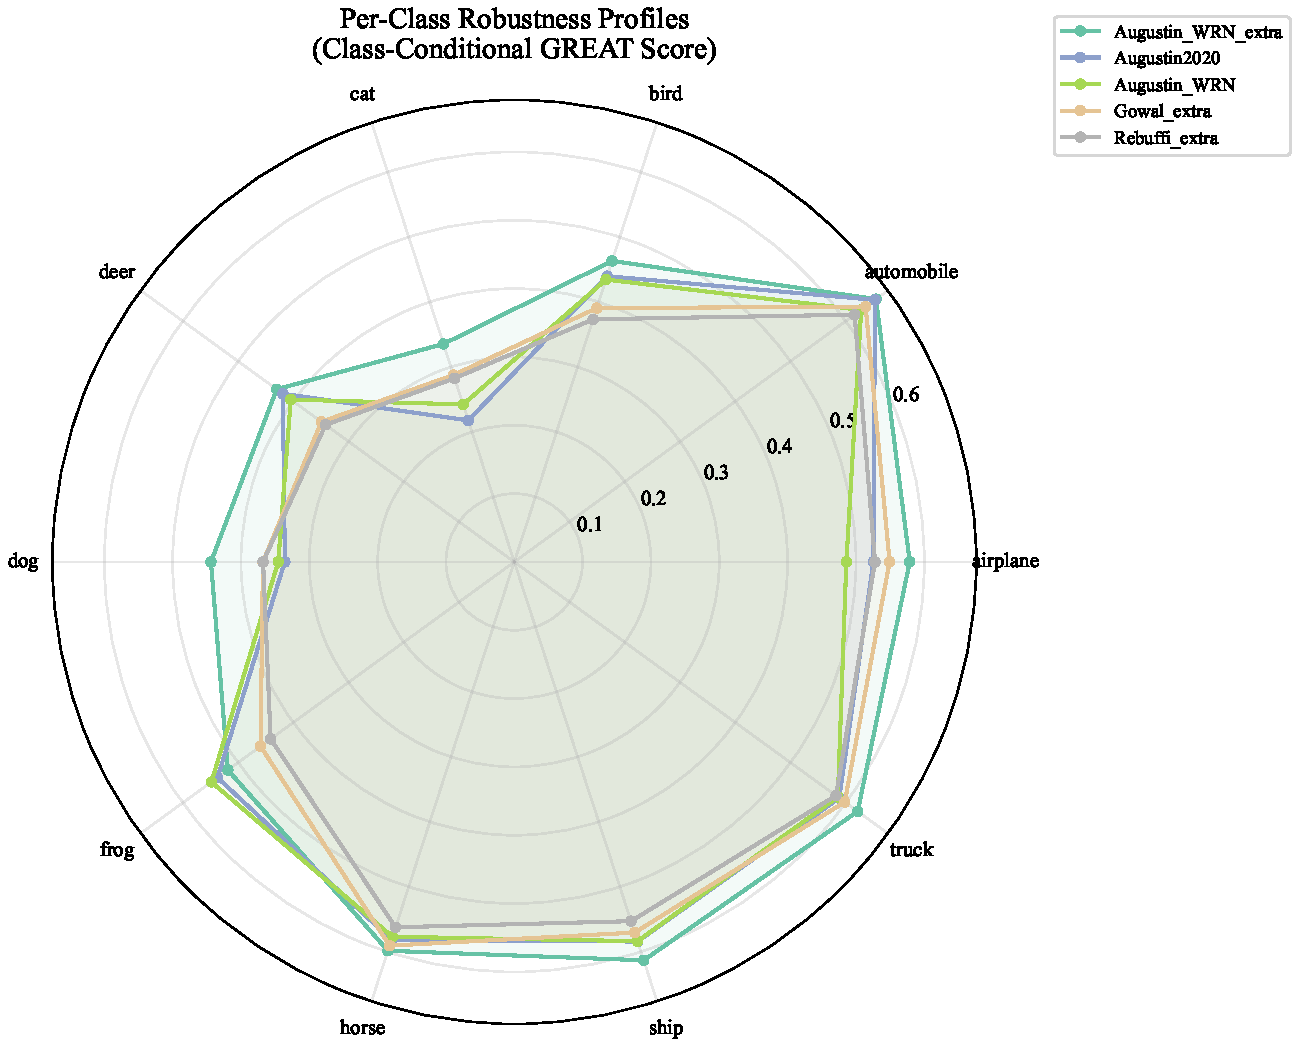
\includegraphics[width=0.7\linewidth]{figures/cifar/radar.pdf}
    \caption{Radar chart of per-class GREAT Scores for selected CIFAR-10 models. Each axis represents one class. Models with higher aggregate scores (outer polygons) show more pronounced asymmetry between classes, visually confirming the robustness-fairness tension.}
    \label{fig:radar_cifar}
\end{figure}

\subsection{ImageNet Heatmap}
\label{app:imagenet_heatmap}

\Cref{fig:heatmap_imagenet} shows the per-class GREAT Score heatmap for ImageNet models, analogous to \Cref{fig:heatmap} in the main text for CIFAR-10.

\begin{figure}[H]
    \centering
    
\includegraphics[width=0.85\linewidth]{figures/imagenet/heatmap.pdf}
    \caption{Per-class GREAT Scores for 5 ImageNet $\ell_\infty$ models. The extreme contrast between the brightest and darkest columns reflects the high RDI values ($> 1.1$) reported in \Cref{tab:imagenet_full}. Several classes receive near-zero scores across all models.}
    \label{fig:heatmap_imagenet}
\end{figure}

\section{Interactive Auditing Dashboard}
\label{app:dashboard}

To bridge the gap between formal metrics and practitioner-friendly evaluation, we develop an interactive auditing dashboard built with Gradio. The dashboard supports both CIFAR-10 and ImageNet evaluation results and provides the following functionality:

\begin{itemize}
    \item \textbf{Dataset and model selection}: Users select a dataset and model from dropdown menus populated with all evaluated models.
    \item \textbf{Adjustable fairness penalty}: A slider controls the $\lambda$ parameter for FP-GREAT, allowing real-time exploration of how the fairness-robustness trade-off affects model ranking.
    \item \textbf{Per-class breakdown}: A detailed table displays per-class GREAT Scores, clean accuracies, and vulnerability rankings for the selected model.
    \item \textbf{Aggregate metrics}: Summary statistics including the aggregate GREAT Score, RDI, NRGC, WCR, and FP-GREAT are displayed prominently.
    \item \textbf{HTML audit report}: A one-click export generates a structured audit report summarizing all metrics and class-level findings for documentation purposes.
\end{itemize}

The dashboard loads pre-computed results from JSON files generated by the evaluation pipeline, requiring no GPU at runtime. It can be launched with \texttt{python -m gf\_score.auditing\_tool.app} and is accessible through any web browser. The tool is designed for model auditors and deployment teams who need to assess whether a model meets class-level robustness requirements before deployment.

% ======================================================================
% CITATION LIST (for bib file generation)
% ======================================================================
% [1] Abid et al. (2019) "Gradio: Hassle-Free Sharing and Testing of ML Models in the Wild"
%     https://arxiv.org/abs/1906.02569
%
